% Options for packages loaded elsewhere
\PassOptionsToPackage{unicode}{hyperref}
\PassOptionsToPackage{hyphens}{url}
%
\documentclass[
]{article}
\usepackage{amsmath,amssymb}
\usepackage{iftex}
\ifPDFTeX
  \usepackage[T1]{fontenc}
  \usepackage[utf8]{inputenc}
  \usepackage{textcomp} % provide euro and other symbols
\else % if luatex or xetex
  \usepackage{unicode-math} % this also loads fontspec
  \defaultfontfeatures{Scale=MatchLowercase}
  \defaultfontfeatures[\rmfamily]{Ligatures=TeX,Scale=1}
\fi
\usepackage{lmodern}
\ifPDFTeX\else
  % xetex/luatex font selection
\fi
% Use upquote if available, for straight quotes in verbatim environments
\IfFileExists{upquote.sty}{\usepackage{upquote}}{}
\IfFileExists{microtype.sty}{% use microtype if available
  \usepackage[]{microtype}
  \UseMicrotypeSet[protrusion]{basicmath} % disable protrusion for tt fonts
}{}
\makeatletter
\@ifundefined{KOMAClassName}{% if non-KOMA class
  \IfFileExists{parskip.sty}{%
    \usepackage{parskip}
  }{% else
    \setlength{\parindent}{0pt}
    \setlength{\parskip}{6pt plus 2pt minus 1pt}}
}{% if KOMA class
  \KOMAoptions{parskip=half}}
\makeatother
\usepackage{xcolor}
\usepackage[margin=1in]{geometry}
\usepackage{graphicx}
\makeatletter
\def\maxwidth{\ifdim\Gin@nat@width>\linewidth\linewidth\else\Gin@nat@width\fi}
\def\maxheight{\ifdim\Gin@nat@height>\textheight\textheight\else\Gin@nat@height\fi}
\makeatother
% Scale images if necessary, so that they will not overflow the page
% margins by default, and it is still possible to overwrite the defaults
% using explicit options in \includegraphics[width, height, ...]{}
\setkeys{Gin}{width=\maxwidth,height=\maxheight,keepaspectratio}
% Set default figure placement to htbp
\makeatletter
\def\fps@figure{htbp}
\makeatother
\setlength{\emergencystretch}{3em} % prevent overfull lines
\providecommand{\tightlist}{%
  \setlength{\itemsep}{0pt}\setlength{\parskip}{0pt}}
\setcounter{secnumdepth}{-\maxdimen} % remove section numbering
\usepackage{booktabs}
\usepackage{longtable}
\usepackage{array}
\usepackage{multirow}
\usepackage{wrapfig}
\usepackage{float}
\usepackage{colortbl}
\usepackage{pdflscape}
\usepackage{tabu}
\usepackage{threeparttable}
\usepackage{threeparttablex}
\usepackage[normalem]{ulem}
\usepackage{makecell}
\usepackage{xcolor}
\ifLuaTeX
  \usepackage{selnolig}  % disable illegal ligatures
\fi
\usepackage{bookmark}
\IfFileExists{xurl.sty}{\usepackage{xurl}}{} % add URL line breaks if available
\urlstyle{same}
\hypersetup{
  hidelinks,
  pdfcreator={LaTeX via pandoc}}

\author{}
\date{\vspace{-2.5em}}

\begin{document}

\section{Fundamentals of Data Science Assessment
Sheet}\label{fundamentals-of-data-science-assessment-sheet}

\paragraph{\texorpdfstring{\emph{Matt
Prill}}{Matt Prill}}\label{matt-prill}

Note: \emph{All code formulated for this assessment is accessible in my
github repository linked here. It also contains images of my hand
written workings out. There is no onus to look at these; all relevant
and neat workings can be seen in this document. I have included them in
the repository so that I can} \textbf{(A)} \emph{track my own workflow
(version control) and} \textbf{(B)} \emph{allow you to consult them
should you wish to.}

\subsection{Question 1a}\label{question-1a}

\paragraph{Initial Equations:}\label{initial-equations}

\[
\Large
\begin{aligned}
x + y + z &= 1 \\
x + 2y + 4z &= \eta \\
x + 4y + 10z &= \eta^2
\end{aligned}
\]\\

\paragraph{Corresponding Coefficient
Matrix:}\label{corresponding-coefficient-matrix}

\[
\Large
A = \begin{bmatrix}
1 & 1 & 1 \\
1 & 2 & 4 \\
1 & 4 & 10 
\end{bmatrix}
\begin{bmatrix}
1  \\
η  \\
η^2  
\end{bmatrix}
\]

\paragraph{Calculating the Determinant of
A:}\label{calculating-the-determinant-of-a}

To showcase that these equations lack a unique solution for any value of
η, I can attempt to find the determinant. To to find a determinant of
square matrix (irrespective of size), I must;

\begin{enumerate}
\def\labelenumi{\arabic{enumi}.}
\tightlist
\item
  Pick a coefficient from the first row.
\item
  Delete remaining elements in coefficient's respective row and column.
\item
  Make a matrix of the remaining elements.
\item
  Find the determinant of the sub-matrix, and multiply this with the
  coefficient.
\item
  Repeat the same procedure for each element in the first row.
\item
  To determine the sign of each term, sum the indices of the
  coefficient. If it is even, the sign is positive, and if it's odd, the
  sign is negative.
\item
  Sum all terms to find the determinant (Linear Algebra Slides, 2019).
\end{enumerate}

Therefore, to find the determinant (\(\text{det}\)) of a \(3 \times 3\)
matrix, I can use the following formula:

\[
\Large
\text{det} \begin{bmatrix} a & b & c \\ d & e & f \\ g & h & i \end{bmatrix} = a \times \text{det} \begin{bmatrix} e & f \\ h & i \end{bmatrix} - b \times \text{det} \begin{bmatrix} d & f \\ g & i \end{bmatrix} + c \times \text{det} \begin{bmatrix} d & e \\ g & h \end{bmatrix}
\]

The terms are added/ subtracted depending on the sum the row and column
indices of the coefficient. Even = positive. Odd = negative. For example
``- b'' is negative because b is \(x_{12}\), thus the sum of the row and
column indices \(= 1+2 = 3 = odd\).

Applying this to the \(3 \times 3\) matrix:

\[
\Large
A = \begin{bmatrix}
1 & 1 & 1 \\
1 & 2 & 4 \\
1 & 4 & 10 
\end{bmatrix}
=
\begin{bmatrix}
a & b & c \\
d & e & f \\
g & h & i 
\end{bmatrix}
\]

Thus,

\[
\Large
\text{det}(A) =
1 \times \text{det} \begin{bmatrix} 2 & 4 \\ 4 & 10 \end{bmatrix} - 1 \times \text{det} \begin{bmatrix} 1 & 4 \\ 1 & 10 \end{bmatrix} + 1 \times \text{det} \begin{bmatrix} 1 & 2 \\ 1 & 4 \end{bmatrix}
\]

To calculate the determinants of the \(2 \times 2\) matrices, I can
apply the formula:

\[
\Large
\text{det}\begin{bmatrix} a & b \\ c & d \end{bmatrix} = ad - bc
\] Corresponding calculations for determinants of the \(2 \times 2\)
matrices:

\[
\Large
\text{det} 
 \begin{bmatrix} 2 & 4 \\ 4 & 10 \end{bmatrix} = 20 - 16 =\mathbf{4}
\]

\[
\Large
 \text{det} \begin{bmatrix} 1 & 4 \\ 1 & 10 \end{bmatrix} = 10 - 4 =\mathbf{6}
\]

\[
\Large
 \text{det} \begin{bmatrix} 1 & 2 \\ 1 & 4 \end{bmatrix} = 4-2 = \mathbf{2}
\]

Substituting these determinants into the aforementioned \(3 \times 3\)
matrix determinant formula gives:

\[
\Large
\text{det}(A)=
(1 \times 4)  - (1 \times 6) + (1 \times 2) = \mathbf{0}
\]

The determinant of the coefficient matrix and therefore the matrix
vector is \(0\). This means that the matrix is singular:

\[
\Large
\text{det}(A) = Ax = 0
\]\\

In being singular, the matrix does not have an inverse meaning that the
corresponding linear equations have either no, or unlimited solutions.
Regardless, in this case, the initial equations have no unique solution
for \(η\).

\hfill\break
\hfill\break
\hfill\break
\hfill\break

\subsection{Question 1b}\label{question-1b}

\paragraph{The Set of Linear
Equations:}\label{the-set-of-linear-equations}

\[
\Large
\begin{aligned}
x + y + z &= 1 \\
x + 2y + 4z &= \eta \\
x + 4y + 10z &= \eta^2
\end{aligned}
\]\\

\paragraph{The Corresponding Augmented
Matrix:}\label{the-corresponding-augmented-matrix}

\[
\Large
\left[
\begin{array}{ccc|c}
1 & 1 & 1 & 1 \\
1 & 2 & 4 & \eta \\
1 & 4 & 10 & \eta^2
\end{array}
\right]
\]

\paragraph{Using Gaussian Elimination to Identify the Solutions for
η:}\label{using-gaussian-elimination-to-identify-the-solutions-for-ux3b7}

\begin{enumerate}
\def\labelenumi{\arabic{enumi}.}
\item
  \[\Large
  (\text{Row }2) -1 \times (1) = 
  \left[
  \begin{array}{ccc|c}
  1 & 1 & 1 & 1 \\
  0 & 1 & 3 & \eta-1 \\
  1 & 4 & 10 & \eta^2
  \end{array}
  \right]
  \]
\item
  \[\Large
   (\text{Row } 3) -1 \times (1) = 
  \left[
  \begin{array}{ccc|c}
  1 & 1 & 1 & 1 \\
  0 & 1 & 3 & \eta-1 \\
  0 & 3 & 9 & \eta^2-1
  \end{array}
  \right]
  \]
\item
  \[\Large
  (\text{Row }3) -3 \times (2) = 
  \left[
  \begin{array}{ccc|c}
  1 & 1 & 1 & 1 \\
  0 & 1 & 3 & \eta-1 \\
  0 & 0 & 0 & \eta^2-3\eta +2
  \end{array}
  \right]
  \]\\
\end{enumerate}

The equation corresponding to the bottom row of the augmented matrix is
0. It is also a quadratic equation where:

\[
\Large
\eta^2-3\eta +2
= ax^2 + bx + c = 0
\]

Now, I can either factorise:

\[
\Large
\eta^2-3\eta +2=
(\eta-1)(\eta-2)= 0
\]

Or alternatively, I can use the quadratic formula to derive the
solutions for \(\eta\):

\[
\Large
\eta = \frac{-b \pm \sqrt{b^2 - 4ac}}{2a}
 = \frac{-(-3) \pm \sqrt{-3^2 - 4\times1\times2}}{2\times1}
 = 1 \text{ or } 2
\]

\hfill\break

\[
\Large
\eta = 1 \text{ or } 2
\]

\hfill\break

\paragraph{Characterising the equations for both
solutions:}\label{characterising-the-equations-for-both-solutions}

\subparagraph{\texorpdfstring{Where
\(\eta = 1\):}{Where \textbackslash eta = 1:}}\label{where-eta-1}

\[
\Large
\begin{aligned}
x + y + z &= 1 \\
x + 2y + 4z &= 1 \\
x + 4y + 10z &= 1^2
\end{aligned}
\]

Corresponding augmented matrix:

\[
\Large
\left[
\begin{array}{ccc|c}
1 & 1 & 1 & 1 \\
0 & 1 & 3 & 1-1 \\
0 & 0 & 0 & 1^2-3(1)\ + 2
\end{array}
\right]
\Large
= 
\left[
\begin{array}{ccc|c}
1 & 1 & 1 & 1 \\
0 & 1 & 3 & 0 \\
0 & 0 & 0 & 0\ 
\end{array}
\right]
\]

Thus, when \(\eta = 1\):

\[
\Large
\begin{aligned}
x + y + z &= 1 \\
y + 3z & = 0 \\
\end{aligned}
\]

\subsection{?Now I can assign the free variable (z) to a parameter and
characterise
?}\label{now-i-can-assign-the-free-variable-z-to-a-parameter-and-characterise}

\hfill\break
\hfill\break
\hfill\break

\subparagraph{\texorpdfstring{Where
\(\eta = 2\):}{Where \textbackslash eta = 2:}}\label{where-eta-2}

\[
\Large
\begin{aligned}
x + y + z &= 1 \\
x + 2y + 4z &= 2 \\
x + 4y + 10z &= 2^2
\end{aligned}
\]

Corresponding augmented matrix:

\[
\Large
\left[
\begin{array}{ccc|c}
1 & 1 & 1 & 1 \\
0 & 1 & 3 & 2-1 \\
0 & 0 & 0 & 2^2-3(2)\ + 2
\end{array}
\right]
\Large
= 
\left[
\begin{array}{ccc|c}
1 & 1 & 1 & 1 \\
0 & 1 & 3 & 1 \\
0 & 0 & 0 & 0\ 
\end{array}
\right]
\]

Thus when \(\eta = 2\):

\[
\Large
\begin{aligned}
x + y + z &= 1 \\
y + 3z & = 1 \\
\end{aligned}
\]

\subsection{?Now I can assign the free variable (z) to a parameter and
characterise?}\label{now-i-can-assign-the-free-variable-z-to-a-parameter-and-characterise-1}

\hfill\break
\hfill\break
\hfill\break
\hfill\break
\hfill\break
\hfill\break

\subsection{Question 2a}\label{question-2a}

\(P_{1} = P(\text{Alice winning when first to throw})\)

The distribution shares some characteristics of the Bernoulli
distribution whereby there are two outcomes (success \& failure) and
discrete. However, the question is asking for the probability to a given
success. The balls are thrown (trials) until a success (hit).
Furthermore, I have to assume that each throw is independent of the
other which makes the distribution memoryless with two outcomes: success
(win), \& failure (miss). This is a geometric distribution.

\[
\large
\left.
\begin{aligned}
\text{Hit} = α\\
\text{Miss}= 1-α\
\end{aligned}
\right\} \text{Alice}
\]

\[
\large
\left.
\begin{aligned}
\text{Hit} =  β\\
\text{Miss}= 1- β\
\end{aligned}
\right\} \text{Ben}
\]

\paragraph{The probability of Alice missing Ben with her first throw and
going on to
win:}\label{the-probability-of-alice-missing-ben-with-her-first-throw-and-going-on-to-win}

P(Alice misses first throw) = \(1 - α\)

P(Ben misses first throw) = \(1-β\)

Thus,\\
P(Alice miss, Ben miss) = \((1 - α)\times (1-β)\)

So,\\
P(Alice miss, Ben miss, Alice goes onto win) =
\(P_{1}\times(1 - α) \times(1 - β)\)

\(P_{1}\) is able to be used here because of the memoryless nature of
the geometric distribution; no matter how many trials have transpired
prior to a given throw of Alice's, the probability that she will win
from that point onwards is still \(P_{1}\).

\hfill\break
\hfill\break

\subsection{Question 2b}\label{question-2b}

Because I'm working with the Geometric distribution with parameter p, X
has a probability mass function:

\[
\large
P(X = k) = p(k) =
\left\{
\begin{aligned}
(1 − p)^{k-1}p,\\
0\
\end{aligned}
\right.
\]

This is not conditional probability as the probability is with respect
to the beginning of the round.

As discussed, the probability that Alice and Ben both miss in a given
round is: \((1 - α)\times (1-β)\)

\hfill\break
This could repeat n times where n can denotes any integer
(theoretically): \(((1 - α)\times (1-β))^n\) meaning the probability
will be a summation of all the rounds where n is potentially indefinite
\((\sum_{n=1}^{\infty})\)

\hfill\break
Eventual success from Alice (given that she throws first) therefore
gives: \[
\Large
P(X = n) =  \sum_{n=1}^{\infty} ((1 - α)\times (1-β))^{n-1} \timesα
\]\\

The \(n-1\) term is used because Alice and Ben must miss every time
until the final round (hence \(-1\)); the \(n\)-th round is the one she
wins (success).

The \(α\) term is therefore added as it still denotes the probability
that she will hit successfully.

\hfill\break
Therefore, substituting my terms in gives:

\[
\Large
P_{1} =  \sum_{n=1}^{\infty} ((1-α)\times(1-β))^{n-1}\times α
\]

In line with the geometric series, this is then equivalent to: \[
\Large
P_{1} =
α\times \sum_{n=0}^{\infty} ((1-α)\times(1-β))^{n}
\] This holds even if n = 0 because in this instance the equation would
still equate to α.\\
\strut \\

In the infinite geometric series equation
\(\sum_{n=0}^{\infty}r^n=\frac{1}{1-r}\) where \(|r|< 1\)\\
\((1-α)\times(1-β)\) is the common ratio (this holds because the terms
are probabilities and so \textless{} 1) Thus:

\[
\Large 
r = (1-α)\times(1-β)
\]\\
\strut \\

Finally, substituting the values into the geometric series equation
gives: \[
\Large
P_{1} = α \times \frac{1}{1-(1-α)\times(1-β)}
\]

\subsection{Question 2c}\label{question-2c}

For Ben to throw go first but Alice still to win, there must be \(1-β\)
term.

However given the order of throws, the point at which Alice wins must be
preceded by a miss from Ben \((1-β)\) after which she can throw (and
win). Therefore,

\[
\Large 
P_{2}\neq \sum_{n=1}^{\infty} ((1-β) \times (1-α))^{n-1} \times α
\]

Instead there must be a final \(1-β\) before Alice is victorious. Again,
the \(n\)-th round is the one where she wins (also the round where Ben
misses a final time) Thus,

\[
\Large 
P_{2} = \sum_{n=1}^{\infty} ((1-β) \times (1-α))^{n-1} \times (1-β) \times α 
\]

By applying the geometric series steps as in the previous question, we
get that: \[
\Large 
P_{2} = (1-β) \times α \times \sum_{n=0}^{\infty} ((1-β) \times (1-α))^{n}
\] And finally:

\[
\Large
P_{2} = (1-β)\timesα \times \frac{1}{1-(1-α)\times(1-β)}
\]\\
\strut \\
\strut \\
\strut \\

\subsection{Question 3a}\label{question-3a}

Infinite geometric series for \(|r| < 1\):\\
\[
\Large 
\sum_{n=0}^{\infty}r^n=\frac{1}{1-r} 
\]\\

The equation \(\sum_{n=0}^{\infty}n(n-1)r^{n-2}\) has no common ratio
i.e.~there are extra terms: \(n(n-1)\) - a polynomial.This means it is
not part of the geometric series. However, I can but we can use
properties of the geometric series to work out the sum of the latter. I
can do so by altering the geomtric series to take the same form of the
equation of interest.

1.Differentiating the geometric series gives a similar form to the
second expression:

\[
\Large
\frac{d}{dx} \left( \sum_{n=0}^{\infty} r^n \right) = \frac{d}{dx} \left( \frac{1}{1 - r} \right)
\]

For the first term (equation) I apply the power rule:
\(\frac{d}{dx} \left( x^n \right) = n x^{n-1}\) Note, I am derivating
with respect to \(r\) i.e.~\(r = x\) to match geometric series form.

\[
\Large
\frac{d}{dx} \left( \sum_{n=0}^{\infty} r^n \right) =
\sum_{n=0}^{\infty} nr^{n-1}
\]

And for the sum I can apply the quotient rule to find the derivative:
\(\frac{d}{dx} \left( \frac{f}{g} \right) = \frac{g \frac{d}{dx}(f) - f \frac{d}{dx}(g)}{g^2}\)
Again, I am derivating with respect to r (r = x)

\[
\Large
 \frac{d}{dx} \left( \frac{1}{1 - r} \right) = \frac{(1-r)\times\frac{d}{dx}(1)-1 \times \frac{d}{dx}(1-r)}{(1-r)^2}
 = \frac{1}{(1-r)^2}
\]

Now I have:

\[
\Large
\sum_{n=0}^{\infty} nr^{n-1} = \frac{1}{(1-r)^2}
\]

The equation form now mirrors that of the equation of interest:
\(\sum_{n=0}^{\infty}n(n-1)r^{n-2}\)

\paragraph{Next, I can take the second
derivative:}\label{next-i-can-take-the-second-derivative}

The second derivative of \(\sum_{n=0}^{\infty}r^n\):

\[
\Large \frac{d^2}{dx^2} \left( \sum_{n=0}^{\infty} r^n \right) = \frac{d}{dx} \sum_{n=0}^{\infty} n r^{n-1}
\]

Using the power rule again:

\[
\Large
\frac{d}{dx}\sum_{n=0}^{\infty} nr^{n-1}
= \sum_{n=0}^{\infty}n(n-1)r^{n-2}
\]

This is the exact same as the equation of interest. Therefore, the
second derivative of the given geometric series
\(( \sum_{n=0}^{\infty} r^n)\) is equal to the equation of interest:

\[
\Large
\frac{d2}{dx2} \left( \sum_{n=0}^{\infty} r^n \right) = \frac{d}{dx}\sum_{n=0}^{\infty} nr^{n-1} = \sum_{n=0}^{\infty}n(n-1)r^{n-2}
\]

Therefore, to find its respective sum, I must find the second derivative
of the initial equations sum too. I can do this again with the quotient
rule.

\[
\Large
\frac{d2}{dx2} \left( \frac{1}{1 - r} \right) =
\frac{d}{dx} \left( \frac{1}{(1 - r^2)} \right) =
\frac{(1-r)^2\times\frac{d}{dx}(1)-1 \times \frac{d}{dx}(1-r)^2}{((1-r)^2)^2}
\]\\
\strut \\
Note: I now also have to apply chain rule to differentiate \((1-r)^2\).
\(1-r\) is the inner function, \(^2\) is the outer. So
\(\frac{d}{dx}(1-r)^2 = -2(1-r)\) Thus, I arrive at:

\hfill\break
\[
\Large
= \frac{(1-r)^2\times0-1 \times (-2\times(1-r))}{(1-r)^4}=\frac{2(1-r)}{(1-r)^4} =\frac{2}{(1-r)^3}
\]

To conclude:

\[
\Large
\sum_{n=0}^{\infty}n(n-1)r^{n-2} =\frac{2}{(1-r)^3}
\]

\hfill\break
\hfill\break
\hfill\break
\hfill\break
\hfill\break

\hfill\break

\hfill\break
\hfill\break
\hfill\break

\hfill\break
\hfill\break
\hfill\break

\subsection{Question 3b}\label{question-3b}

\subsubsection{A:}\label{a}

I need to calculate the expectation of a fine (true when weight \(<\)
420.75) per box. This is equivalent to the CDF \(F(x) = P(X ≤ 420.75)\).
Then I can calculate the expected value of the fine/box.

The tins weight follows a normal distribution
\(X\text~N(μ = 426, σ = 21)\). The PDF of the normal distribution is:

\[
\Large
f(x \mid \mu, \sigma^2) = \frac{1}{2 \pi \sigma^2} \exp \left\{ -\frac{1}{2 \sigma^2} (x - \mu)^2 \right\}
\]

Substituting the parameters gives:

\[
\Large
f(x \mid 426, 21^2)  = \frac{1}{2 \pi (21)^2} \exp \left\{ -\frac{1}{2 \times (21)^2} (x - 426)^2 \right\}
\]

The corresponding CDF cannot be denoted analytically due to but must be
evaluated. The CDF \(F(x) = P(X ≤ 420.75)\) is the integral of the PDF.
However, the CDF of a normal distribution (denoted as \(\Phi\)) which
means I can consult a `Z-' probability table. To calculate the CDF
corresponding z-value I can use the formula:

\[
\Large
Z = \frac{X - \mu}{\sigma_{\text{sample}}}
\]

Importantly, the variance value in this term is actually standard
deviation of a box because it is tied to the sample size. In this case,
the sample size is a whole box (100 cans), not a single tin:

\[
\Large
\sigma_{\text{sample}} = \frac{\sigma}{\sqrt{n}} = \frac{21}{\sqrt{100}} = 2.1
\] This makes sense because as sample size increases, variance should
decrease. In turn, by weighing a whole box, the variance of the box will
decrease significantly, even if the variance of the individual tins is
constant.\\

Substituting the parameters into the penultimate equation gives:

\[
\Large
Z = \frac{420.75 - 426}{2.1} = -2.50
\]\\

\paragraph{Now, I can consult the
z-table:}\label{now-i-can-consult-the-z-table}

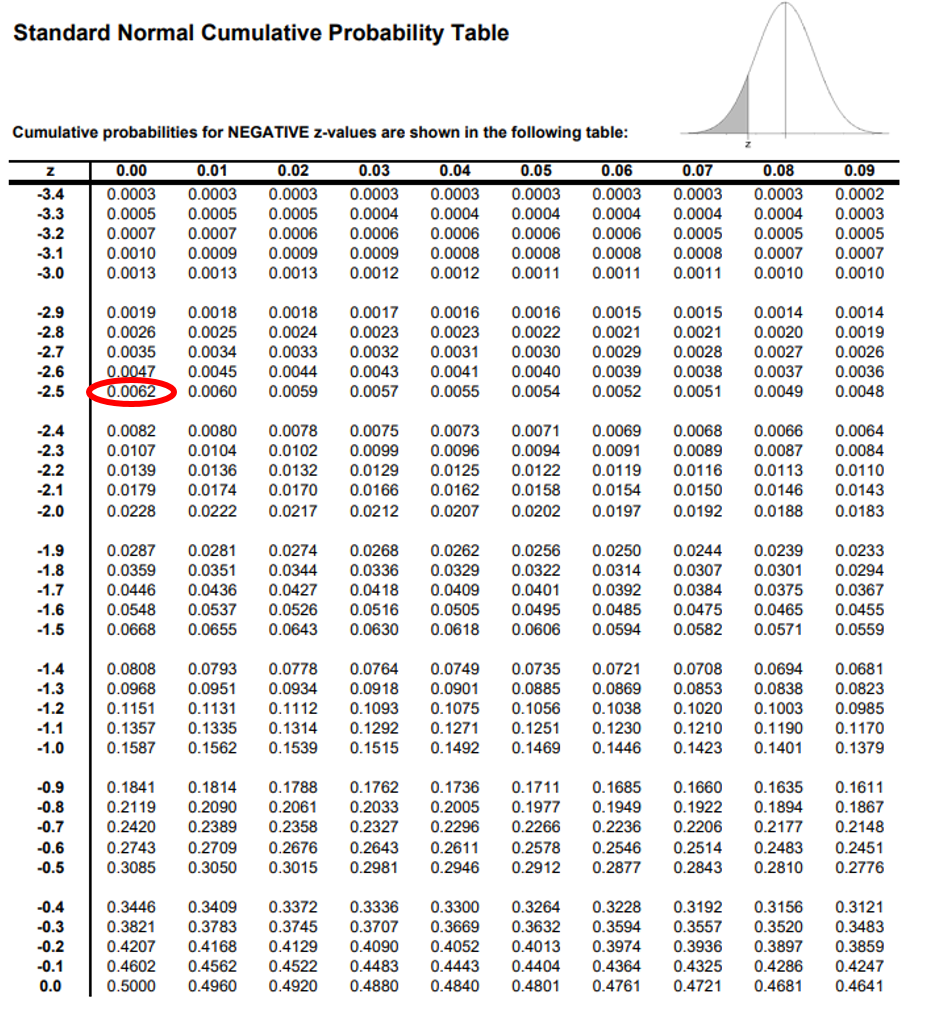
\includegraphics{images/ztable.png}\\
The CDF's corresponding z-value is 0.0062. This means the probability of
a box's weight/can being \textless420.75g is 0.62\%. To work out the
expectation of the fine:

\[
\Large
E(\text{Fine}) = 3000 \times 0.0062 = 18.6
\]

Thus for A:

\[
\Large
E(\text{Fine})=£18.60\text{/box}
\]\\
\strut \\
\strut \\
\strut \\
\strut \\

\subsubsection{B:}\label{b}

I need to calculate the CDF \(F(x) = P(X ≤ 421.8)\). I will use the same
logic as before and calculate the z-value before consulting the table.
This time, \(X = 421.8\) and \(n = 25\) which means that to calculate
the z-value: \[
\Large
\sigma_{\text{sample}} = \frac{\sigma}{\sqrt{n}} = \frac{21}{\sqrt{25}} = 4.2
\] This higher \(\sigma\) compared to the previous question is to be
expected given the smaller sample size. Thus:

\[
\Large
Z = \frac{421.8 - 426}{4.2} = -1
\]\\

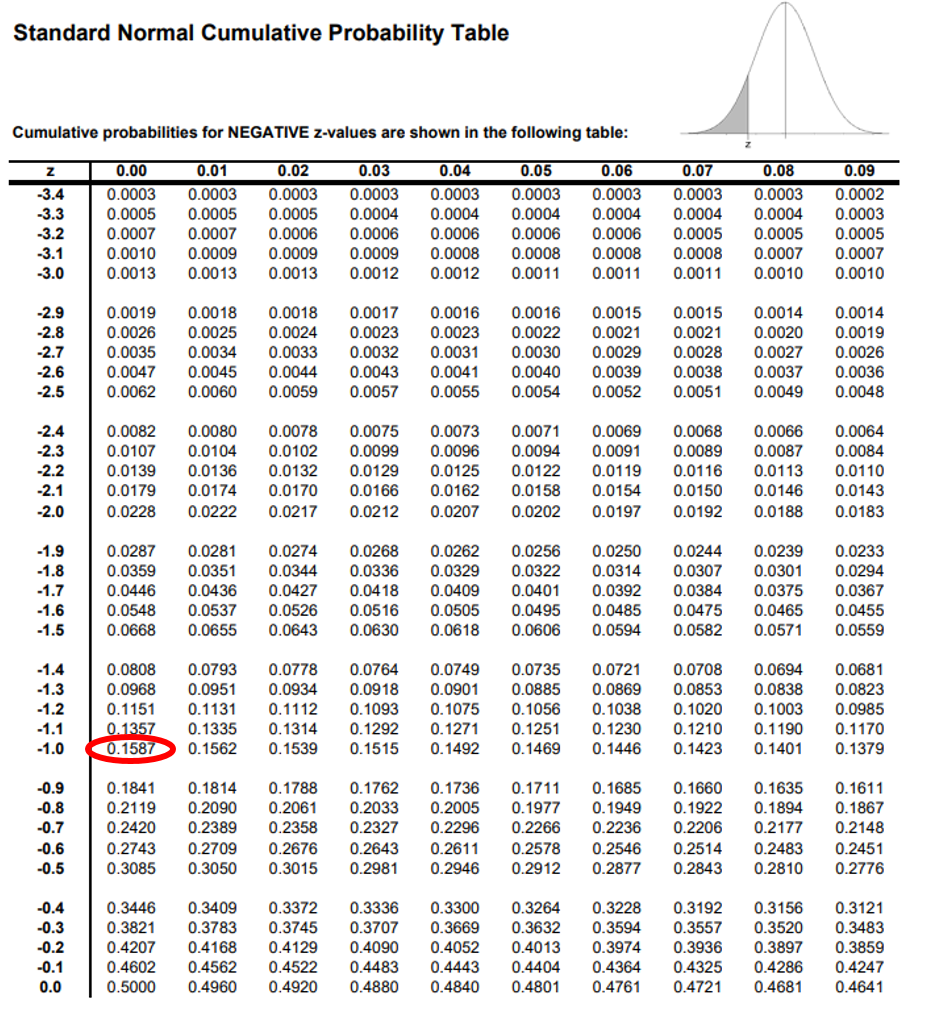
\includegraphics{images/ztableb.png}\\
The CDF's corresponding z-value is 0.1587. This means the probability of
a box's weight/can being \textless421.8g is 15.87\%. To work out the
expectation of the fine:

\[
\Large
E(\text{Fine}) = 120 \times 0.1587 = 19.044
\]

Thus for B:

\[
\Large
E(\text{Fine})=£19.04\text{/box}
\]\\
\strut \\
\strut \\
\strut \\
\strut \\

\subsubsection{C:}\label{c}

The probability that X \textgreater{} 426 is equivalent to
\(1- P(X ≤ 426)\). I could do this again and consult the z-table but
this is unnecessary. 426 is the mean and normally distributed so there
is a 0.5 chance that a randomly sampled can will weigh more and 0.5 that
it will weigh less. Note: this takes into account the fact that a PDF of
a given continuous variable (in this case 426.0g) = 0.

Here, each sampling event is either success \((X > 426)\) or failure
\((X ≤ 426)\) where n could take any number. This is characteristic of
the geometric formula. As discussed, the finite geometric series is:

\[
\Large 
\sum_{n=0}^{\infty}r^n=\frac{1}{1-r} 
\]\\

Since the probability of success = 0.5:

\[
\Large
\sum_{n=0}^{\infty}r^n=\frac{1}{1-0.5}  = 2
\] As expected, it takes two trials until a success is expected. In
turn:

\[
\Large
E(n) = 2
\]

N itself however will have its own distribution which must be considered
before plugging into the fine equation. The variance of n can be
calculated using the varience formula for geometric distributions:

\[
\Large
Var(n) = \frac{1-p}{p^2}
\] Thus, \[
\Large
Var(n) = \frac{1-0.5}{0.5^2}= 2
\]\\

To calculate the expectation of the fine I need to use the formula, \[
\Large
E(n^2) = \text{Var}(n) + (E(n))^2
\]

I have the variance and expected no. samples until success but i also
need the expectation of n\^{}2 becuase \(n(n−1)=n^2−n\). Therefore to
calculate the expectation of \(n^2\):

\[
\Large
E(n)^2 = 4 + 2^2 = 6
\] Now I can calculate the E(n(n-1)):

\[
\Large
E(n(n-1))=  E(n^2) - E(n) = 6-2 = 4
\] Now I have \(E(n(n-1))\), I can plug it into the equation: \[
\Large
E(\text{Fine}) = 5\times{}E(n(n-1))=  5 \times 4 = 20
\] In conclusion: \[
\Large
E(\text{Fine}) =  £20
\]

\[
\Large
E(\text{Fine})= (5n(n−1))
\]\\
\strut \\
\strut \\
\strut \\
\strut \\

\subsection{Question 4a}\label{question-4a}

\paragraph{Introducing the random
variables:}\label{introducing-the-random-variables}

The random variables follow Bernoulli distributions because its
success/failure (outcomes sum to 1), is independent and n is known. It
is not repeated n times for each sample \((i)\). If this were the case
then the distribution would become binomial.

\[
\Large
X_i^{(1)} = \left\{
\begin{array}{ll}
1, & \text{if B supporter number } i \text{ still supports B at the end of day 1}, \\
0, & \text{if B supporter number } i \text{ changes to an M supporter at the end of day 1}.
\end{array}
\right.
\] This is equivalent to:

\[
\Large
X_i^{(1)} = \left\{
\begin{array}{ll}
k= 1, \text{ }p = 1- 0.004 = 0.996 \\
k= 0, \text{ }1-p = 1- 0.996 = 0.004
\end{array}
\right.
\] Each random variables can be denoted as
\(X_i^{(1)} \sim \text{Bernoulli}(p) \text{ for } i = 1...,175\).\\

For \(X^{(2)}\): \[
\Large
X_i^{(2)} = \left\{
\begin{array}{ll}
1, & \text{if M supporter number } i \text{ changes to a B supporter at the end of day 1}, \\
0, & \text{if M supporter number } i \text{ still supports M at the end of day 1}.
\end{array}
\right.
\]

This is equivalent to:

\[
\Large
X_i^{(1)} = \left\{
\begin{array}{ll}
k=1, \text{ }p = 0.005 \\
k=0, \text{ }1-p = 1- 0.005 = 0.996
\end{array}
\right.
\] Again, each random variables can be denoted as \$ X\_i\^{}\{(2)\}
\sim \text{Bernoulli}(p) \text{ for } i = 1\ldots,186\$.\\

\subsubsection{\#\# References}\label{references}

Linear Algebra Slides, 2020

\end{document}
